

\definecolor{sapphire}{rgb}{0.03, 0.15, 0.4}
\definecolor{indigo}{rgb}{0.13, 0.67, 0.8}


\begin{figure}[h]
    \centering
    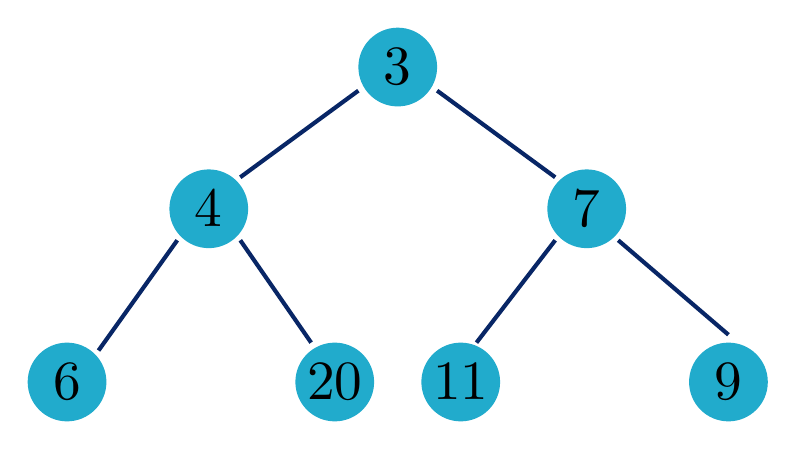
\begin{tikzpicture}[scale=0.4]
        
        %\draw [help lines] (-12,-12) grid (12,12);
        %\draw [sapphire,line width=0.75pt] (10,0) -- (-10,0);
        %\draw [sapphire,line width=0.75pt] (0,10) -- (0,-10);
        
        \path[fill=indigo,line width=1.5pt] (0,5) circle [radius=1.25];
        
        \path[fill=indigo,line width=1.5pt] (-6,0.5) circle [radius=1.25];
        \path[fill=indigo,line width=1.5pt] (6,0.5) circle [radius=1.25];
        
        \path[fill=indigo,line width=1.5pt] (-10.5,-5) circle [radius=1.25];
        \path[fill=indigo,line width=1.5pt] (10.5,-5) circle [radius=1.25];
        \path[fill=indigo,line width=1.5pt] (-2,-5) circle [radius=1.25];
        \path[fill=indigo,line width=1.5pt] (2,-5) circle [radius=1.25];
        
        
        
        \draw [sapphire,line width=1.5pt] (-1.25,4.25) -- (-5,1.5);
        \draw [sapphire,line width=1.5pt] (1.25,4.25) -- (5,1.5);
        
        \draw [sapphire,line width=1.5pt] (-7,-0.5) -- (-9.5,-4);
        \draw [sapphire,line width=1.5pt] (-5,-0.5) -- (-2.75,-3.75);
        
        \draw [sapphire,line width=1.5pt] (7,-0.5) -- (10.5,-3.5);
        \draw [sapphire,line width=1.5pt]  (5,-0.5) -- (2.5,-3.75);
        
        
        
        
        \node[scale = 2] at (0,5) {3};
        
        \node[scale = 2] at (-6,0.5) {4};
        \node[scale = 2] at (6,0.5) {7};
        
        \node[scale = 2] at (-10.5,-5){6};      
        \node[scale = 2] at (10.5,-5) {9};
        \node[scale = 2] at (-2,-5) {20};
        \node[scale = 2] at (2,-5) {11};
        

        
        
        
    \end{tikzpicture}
    \caption{Graph }
\end{figure}